% SEGMENT OLP-0044-S01
% Part: sets-functions-relations
% Chapter: arithmetization
% Section:reals

\documentclass[../../../include/open-logic-section]{subfiles}

\begin{document}

\olfileid{sfr}{arith}{real}
\olsection{மெய்யெண் கோடு}

விகிதமுறு எண்களிலிருந்து மெய்யெண்களை எவ்வாறு கட்டமைப்பது எனக்
காட்டுவது அடுத்த படி. அதற்கு முன், மெய்யெண்களின்
\emph{தனிச்சிறப்பை} நாம் புரிந்துகொள்ள வேண்டும்.

மெய்யெண்கள் விகிதமுறு எண்களைப் பெரிதும் ஒத்துச் செயல்படுகின்றன.
(தொழில்நுட்பமாக, இரண்டுமே \emph{வரிசைப்படுத்தப்பட்ட புலங்களுக்கான}
எடுத்துக்காட்டுகள்; இதன் வரையறைக்கு \olref[check]{orderedfield} ஐப்
பார்க்கவும்.)
\olref[sfr][siz][]{chap} இன் பயிற்சிகளை நீங்கள் செய்திருந்தால்,
விகிதமுறு எண்களைவிடக் கண்டிப்பாக அதிகமான மெய்யெண்கள் உள்ளன,
அதாவது $\cardless{\Rat}{\Real}$, என்பது உங்களுக்குத் தெரியும்.
இதனை முதன்முதலில் காண்டோர் நிறுவினார்.
ஆனால் விகிதமுறா எண்கள், அதாவது விகிதமுறு எண்களாக இல்லாத மெய்யெண்கள்,
இருப்பது ஏறத்தாழ இரண்டாயிரத்து ஐந்நூறு ஆண்டுகளாக அறியப்பட்டுள்ளது.
உண்மையில்:
%\footnote{இப்போது: ``$\sqrt{2}$'' என்பது நேர்ம, எதிர்ம மூலங்கள் இரண்டையும் சமமாகக் குறிக்கிறது; ஆனால் அடுத்த சில பக்கங்களில் இதனை மறந்து, நேர்ம மூலத்தை மட்டும் கருதுவேன்.}

% SEGMENT OLP-0044-S02
\begin{thm}\ollabel{root2irrational}
$\sqrt{2}$ என்பது விகிதமுறு எண் அல்ல;
அதாவது $\sqrt{2} \notin \Rat$.
\end{thm}

% SEGMENT OLP-0044-S03
\begin{proof}
முரண் பெறும் நோக்கில், $\sqrt{2}$ விகிதமுறு எண் எனக் கொள்க.
எனவே ஏதோ இயல் எண்கள் $m$, $n$ ஆகியவற்றுக்கு
$\sqrt{2} = \nicefrac{m}{n}$.
உண்மையில், அந்தப் பின்னத்தை மேலும் சுருக்க முடியாதவாறு
$m$, $n$ ஆகியவற்றைத் தேர்ந்தெடுக்கலாம்.
மறுசீரமைத்தால், $m^{2} = 2n^{2}$.
இங்கிருந்து நிறுவலை இரண்டு வழிகளில் முடிக்கலாம்:

\emph{முதலில், வடிவியலாக} (டென்னன்பாமைப் பின்பற்றி).
\footnote{இந்த நிறுவலை \cite{Conway2006} பதிவுசெய்கிறது.}
இந்த வர்க்கங்களைக் கருதுக:
\begin{center}	
	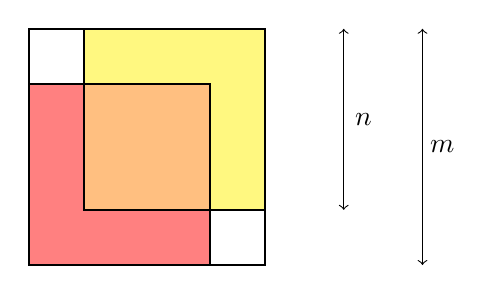
\begin{tikzpicture}
		\draw[thick] (0,0) rectangle (3,3);
		\draw[thick, fill=red!50] (0,0) rectangle (2.3,2.3);
		\draw[thick, fill=yellow!50] (0.7,0.7) rectangle (3, 3);
		\draw[thick, fill=orange!50] (0.7,0.7) rectangle (2.3, 2.3);
		\draw[<->] (4, 0.7)--(4, 3);
		\node at (4.25, 1.85) (n) {$n$};
		\draw[<->] (5, 0)--(5, 3);
		\node at (5.25, 1.5) (m) {$m$};
	\end{tikzpicture}
\end{center}
$m^2 = 2n^2$ என்பதால், $n$ பக்க அளவுள்ள இரண்டு வர்க்கங்களும்
ஒன்றின்மேல் ஒன்று படியும் பகுதியின் பரப்பளவு,
அந்த இரு வர்க்கங்களும் மூடாத பகுதியின் பரப்பளவுக்குச் சமமாகும்;
அதாவது, செம்மஞ்சள் வர்க்கத்தின் பரப்பளவு,
நிறமிடாத இரு வர்க்கங்களின் பரப்பளவுகளின் கூட்டுத்தொகைக்குச் சமம்.
எனவே செம்மஞ்சள் வர்க்கத்தின் பக்க அளவு $p$ ஆகவும்,
நிறமிடாத ஒவ்வொரு வர்க்கத்தின் பக்க அளவு $q$ ஆகவும் இருந்தால்,
$p^2 = 2q^2$.
ஆனால் இப்போது $\sqrt{2} = \nicefrac{p}{q}$;
மேலும் $p < m$, $q < n$, $p, q \in \Nat$.
$m$, $n$ ஆகியவை இயன்றளவு சிறியவையாகத் தேர்ந்தெடுக்கப்பட்டன
என்ற உண்மைக்கு இது முரணாகும்.
		
\emph{இரண்டாவதாக, முறைப்படியாக.}
$m^{2} = 2n^{2}$ என்பதால், $m$ இரட்டை எண் எனப் பின்தொடரும்.
($x$ ஒற்றை எனில், $x^2$ உம் ஒற்றை எனக் காட்டுவது எளிது.)
எனவே ஏதோ ஒரு $r \in \Nat$ க்கு $m = 2r$.
மறுசீரமைத்தால், $2r^2 = n^2$,
		% 				\begin{align*}
		% 					(2q)^{2} &= 2n^{2}\\
		% 					4q^{2} &= 2n^{2}\\
		% 					2q^{2} &= n^{2}
		% 				\end{align*}
எனவே $n$ உம் இரட்டை எண்.
ஆகவே $m$, $n$ இரண்டும் இரட்டை எண்கள்;
இதனால் $\nicefrac{m}{n}$ என்ற பின்னத்தை மேலும் \emph{சுருக்க முடியும்}.
முரண்!
\end{proof}

% SEGMENT OLP-0044-S04
% READER FALLBACK TA-READER-REF-001; absent history chapter gets descriptive text.
இடைச்செய்தியாக, இந்தப் படவிளக்க நிறுவல்
\oliflabeldef{his:set:mythology:sec}{%
  \olref[his][set][mythology]{sec} இன் உள்ளடக்கத்தை}{%
  கணக்கோட்பாட்டு வரலாற்றுக் கதைகள் பற்றிய பின்னைய பிரிவின் உள்ளடக்கத்தை}
மீண்டும் கருத
அனுமதிக்கிறது.
டென்னன்பாம் (1927--2006) முற்றிலும் நவீன கணிதவியலாளர்;
ஆனால் இந்த நிறுவல் மறுக்க முடியாத அளவு அழகானது,
முழுமையாகக் கடுமையானது, வடிவியல் உள்ளுணர்வைப் பயன்படுத்துவது!

% SEGMENT OLP-0044-S05
எப்படியாயினும், மெய்யெண்கள் விகிதமுறு எண்களைவிட
``மேலும் விரிவானவை''.
ஒரு பொருளில், விகிதமுறு எண்களில் ``இடைவெளிகள்'' உள்ளன;
மெய்யெண்கள் அவற்றை நிரப்புகின்றன.
இது விகிதமுறு எண்களிலிருந்து மெய்யெண்களை வேறுபடுத்தும்
மெய்யெண்களின் ஒரே ஒரு பண்பை விவரிப்பதாக வயர்ஸ்ட்ராஸ் உணர்ந்தார்;
அதுவே முழுமைப் பண்பு:
\emph{மேல்வரம்பைக் கொண்ட, வெற்றற்ற மெய்யெண் கணம் ஒவ்வொன்றும்
ஒரு மீச்சிறு மேல்வரம்பைக் கொண்டுள்ளது.}

% SEGMENT OLP-0044-S06
விகிதமுறு எண்களுக்கு முழுமைப் பண்பு இல்லை என்பதை எளிதில் காணலாம்.
எடுத்துக்காட்டாக, $\sqrt{2}$ ஐ விடச் சிறிய விகிதமுறு எண்களைக் கொண்ட
பின்வரும் கணத்தைக் கருதுக:
\[
	\Setabs{p \in \Rat}{p^2 < 2 \text{ அல்லது }p < 0}
\]
இதற்கு விகிதமுறு எண்களில் ஒரு மேல்வரம்பு உள்ளது;
எடுத்துக்காட்டாக, அதன் !!{element}s< அனைத்தும் $3$ ஐ விடச் சிறியவை.
ஆனால் இதன் மீச்சிறு மேல்வரம்பு எது?
அது `$\sqrt{2}$' என்று கூற விரும்புகிறோம்;
ஆனால் $\sqrt{2}$ \emph{விகிதமுறு எண் அல்ல} என்பதை இப்போதுதான் கண்டோம்.
$\sqrt{2}$ ஐ விடப் பெரிய விகிதமுறு எண்களில் \emph{மீச்சிறியது} எதுவும் இல்லை.
எனவே அந்தக் கணத்திற்கு ஒரு மேல்வரம்பு உள்ளது;
ஆனால் மீச்சிறு மேல்வரம்பு இல்லை.
ஆகவே விகிதமுறு எண்களுக்கு முழுமைப் பண்பு இல்லை.

% SEGMENT OLP-0044-S07
இதற்கு மாறாக, தொடரகம் முழுமைப் பண்பைக் கொண்டிருக்க
``கருத்தளவில் வேண்டும்''.
$\sqrt{2}$ ஒரு மெய்யெண்ணாக இருக்க வேண்டும் என்பது மட்டும் நமது நோக்கமல்ல;
விகிதமுறு எண் கோட்டிலுள்ள எல்லா ``இடைவெளிகளையும்'' நிரப்ப விரும்புகிறோம்.
உண்மையில், தொடரகத்திலேயே ``இடைவெளிகள்'' எதுவும் இருக்கக்கூடாது
என விரும்புகிறோம். முழுமை நமக்குத் தருவது இதுவே.

\end{document}
